\begin{scanpage}{0128}{111}
\noindent\begin{minipage}[t]{.48\linewidth}\vspace{0pt}\centering
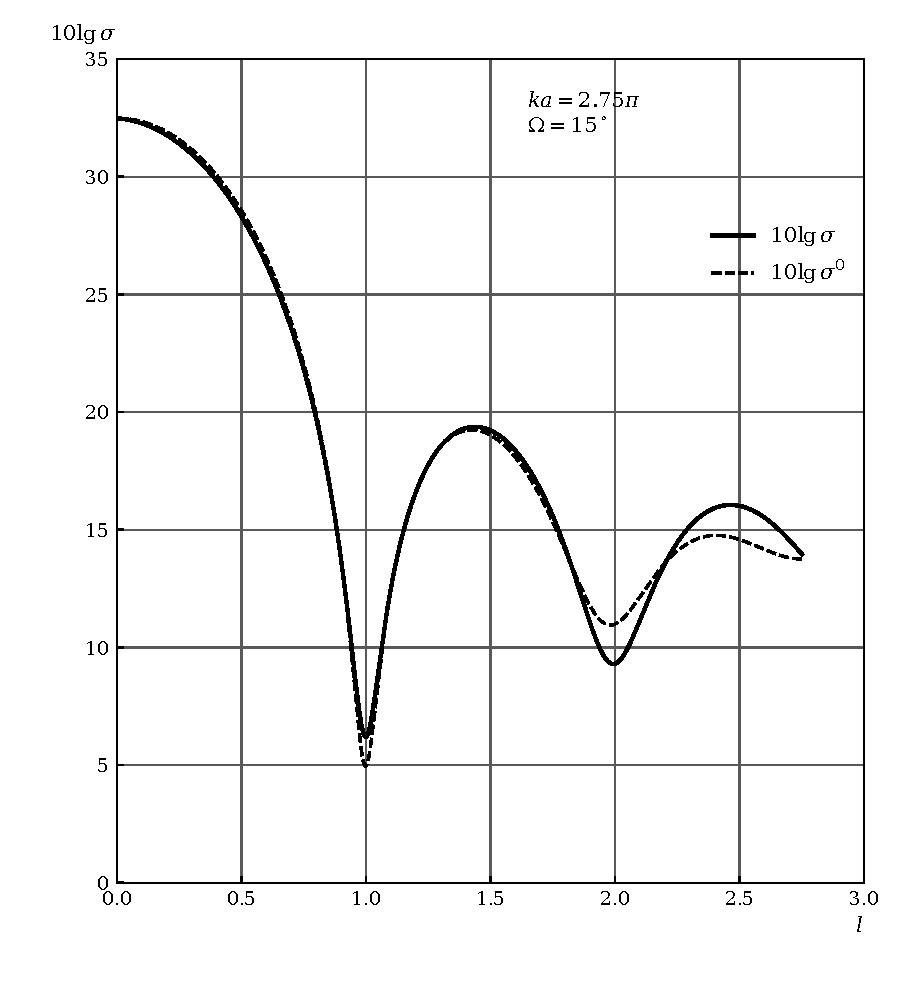
\includegraphics[width=.87\linewidth]{images/recreated/b-0128-fig43.pdf}

\raggedright Figure 43. The effective scattering area of a spherical segment as a function of its length with a constant radius of the base. The function $\sigma$ (the continuous line) is calculated on the basis of Equation (19.12) which considers the nonuniform part of the current near the discontinuity. The function $\sigma^0$ (the dashed line) is calculated from Equation (19.13), and corresponds to the physical optics approach.
\end{minipage}\hfill\begin{minipage}[t]{.48\linewidth}\vspace{0pt}\centering
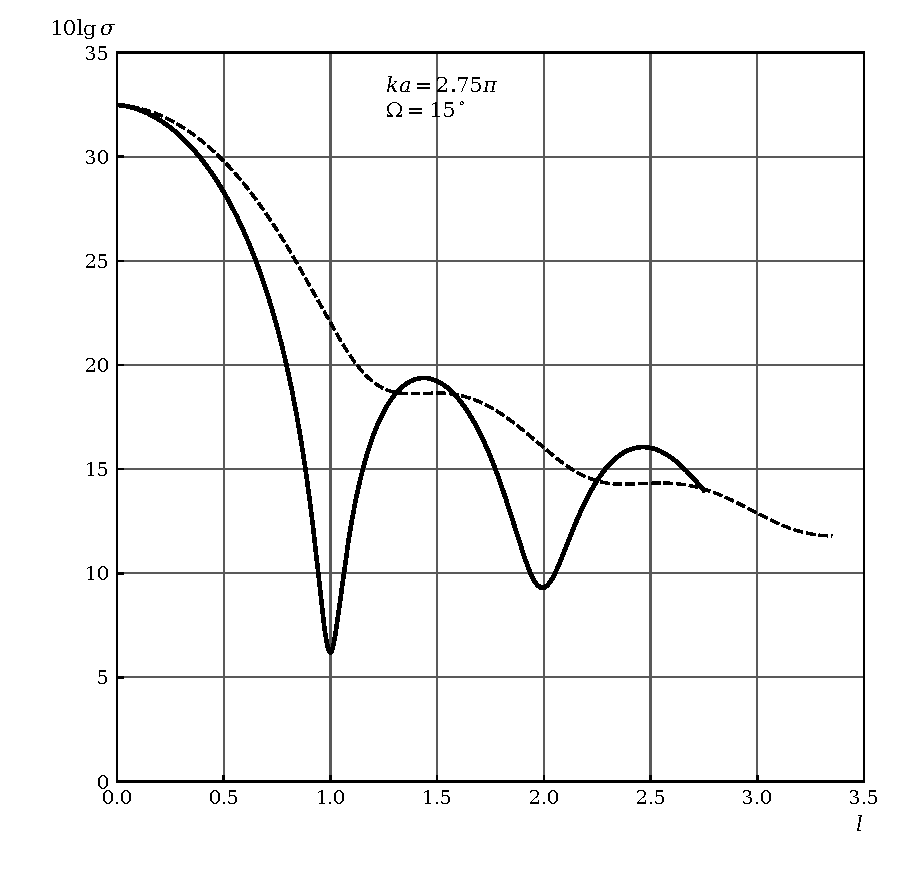
\includegraphics[width=.98\linewidth]{images/recreated/b-0128-fig44.pdf}

\raggedright Figure 44. A comparison of the effective scattering area of a spherical segment (continuous line) and a finite cone (dashed line) which have the same bases.

\vspace{2em}
spherical segment and a finite cone (the dashed curve) which have the same diameter and base shape.
\end{minipage}
\begin{center}$*\quad*\quad*\quad*\quad*\quad*$\end{center}
The results obtained in this Chapter show that the reflected signal depends substantially on the shape of the shaded part of the body, and increases with an increase of the concavity. However, since the nonuniform part of the current is concentrated mainly near the discontinuity, that part of the shaded surface which is several wavelengths away from the discontinuity evidently will not have a noticeable effect on the reflected signal and may be an arbitrary shape.
\end{scanpage}
